%=============================================================================
\section{Introduction and General Overview}
%=============================================================================
\label{sec:introduction}
\noindent
The development of a coherent set of software tools for the description of 
High Energy Physics detectors from a single source of information has been
on the agenda of many experiments for decades.
Providing appropriate and consistent detector views to simulation, 
reconstruction and analysis applications from a single information source
is crucial for the success of the experiments.
Detector description in general includes not only the geometry and the 
materials used in the apparatus, but all parameters describing e.g. the 
detection techniques, constants required by alignment and calibration, 
description of the readout structures, conditions data, etc. 

\noindent
The design of the DD4hep toolkit\cite{bib:DD4hep} 
is shaped on the experience of detector description 
systems, which were implemented for the LHC experiments, in particular 
the LHCb experiment~\cite{bib:LHCb,bib:LHCb-geometry}, 
as well as the lessons learnt from other
implementations of geometry description tools developed for 
the Linear Collider community~\cite{bib:ILD,bib:SiD}. 
Designing a coherent set of tools, with most of the basic components 
already existing in one form or another, is an opportunity for getting 
the best of all existing solutions. 
DD4hep aims to widely reuse used existing software components, in particular
the ROOT geometry package~\cite{bib:ROOT-tgeo}, part of the 
ROOT project\cite{bib:ROOT}, a tool for 
building, browsing, navigating and visualizing detector geometries. The
code is designed to optimize particle transport through complex 
structures and works standalone with respect to any Monte-Carlo 
simulation engine. The ROOT geometry package provides
sophisticated 3D visualization functionality, which is ideal for building 
detector and event displays. The second component is 
the Geant4 simulation toolkit~\cite{bib:geant4}, which is used to 
simulate the detector response from particle collisions in complex designs.
In DD4hep the geometrical
representation provided by ROOT is the main source of information.
In addition DD4hep provides the automatic conversions to other geometrical 
representations, such as Geant4, and the convenient usage of these 
components without the reinvention of the existing functionality.

\noindent
In Section~\ref{sec:architectural-concepts} the scope and the high-level 
requirements of the DD4hep toolkit are elaborated (in the following 
also called "the toolkit"). This is basically the high level vision 
of the provided functionality to the experimental communities. 
In Section~\ref{sec:toolkit-design} the high-level or architectural design 
of the toolkit is presented, and in subsequent subsections design 
aspects of the various functional components and their interfaces will be
introduced.

%=============================================================================
\subsection{Project Scope and Requirements}
%=============================================================================
\label{sec:architectural-concepts}
\noindent
The detector description should fully describe and qualify 
the detection apparatus and must expose access to all information
required to interpret event data recorded from particle collisions.
Experience from the LHC experiments has shown that a generalized
view, not limited only to geometry, is very beneficial in order to obtain 
a coherent set of tools for the interpretation of collision data.
This is particularly important in later stages of the experiment's life cycle,
when a valid set of detector data must be used to analyze real or simulated 
detector response from particle collisions. An example would be an alignment 
application, where time dependent precise detector positions are matched 
with the detector geometry.

\noindent
The following main requirements influenced the design of the toolkit:
\begin{itemize}
\item {\bf{Full Detector Description.}} The toolkit should be able to 
    manage the data describing the detector geometry, the materials used 
    when building the structures, 
    visualization attributes, detector readout information, alignment,
    calibration and environmental parameters - all that is
    necessary to interpret event data recorded from particle collisions.
\item {\bf{The Full Experiment Life Cycle}} should be supported.
    The toolkit should support the development of the detector concepts, 
    detector optimizations, 
    construction and later operation of the detector.
    The transition from one phase to the next should be simple and not require 
    new developments. The initial phases are characterized by very $ideal$
    detector descriptions, i.e. only very few parameters are sufficient 
    to describe new 
    detector designs. Once operational, the detector will be different 
    from the ideal detector, and each part of the detector will have 
    to have its own specific parameters and conditions, 
    which are exposed by the toolkit.
\item {\bf{One single source of detector information}} must be sufficient
    to perform all data processing applications such as simulation, 
    reconstruction, online trigger and data analysis. 
    This ensures that all applications see a coherent description.
    In the past attempts by experiments to re-synchronize parallel
    detector descriptions were always problematic.
    Consequently, the detector description is the union of the information 
    needed by all applications, though the level of detail may be selectable.
\item {\bf{Ease of Use}} influenced both
    the design and the im\-ple\-men\-tation. The definition of sub\-detectors,
    their geometrical description and the access to con\-ditions and alignment 
    data should follow a minimalistic, simple and intuitive interface.
    Hence, the of the developer using the toolkit is focused on specifics of 
    the detector design and not on technicalities handled transparently by 
    the toolkit.
\end{itemize}

%=============================================================================
\begin{figure}[h]
  \begin{center}
    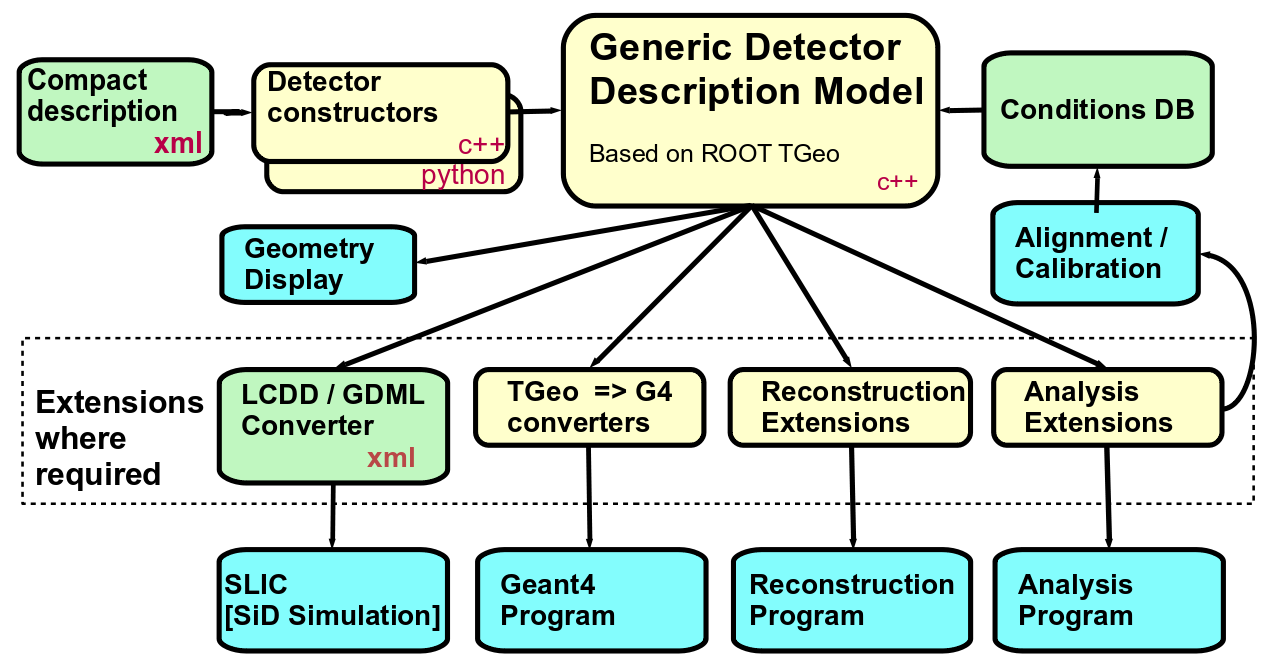
\includegraphics[height=80mm] {DD4hep_big_picture.png}
    \caption{The components of the DD4hep detector geometry toolkit.}
    \label{fig:dd4hep-big-picture}
  \end{center}
  \vspace{-0.4cm}
\end{figure}

%=============================================================================
\subsection{Toolkit Design}
\label{sec:toolkit-design}
%=============================================================================
\noindent
Figure~\ref{fig:dd4hep-big-picture} shows the architecture 
of the main components of the toolkit and their interfaces 
to the end-user applications, namely the simulation, reconstruction, 
alignment and visualization. 
The central element of the toolkit is the so-called generic detector 
description model. This is an in-memory model, i.e., a set of C++ objects 
holding the data describing the geometry and other information of 
the detector. The rest of the toolkit consists of tools and interfaces 
to input or output information from this generic detector model. 
The model and its components will be described in subsequence sections.

%=============================================================================
\subsubsection{The Compact Detector Description}
\label{sec:problem_analysis}
%=============================================================================
\noindent
Inspired from the work of the linear collider detector 
simulation~\cite{bib:LCDD,bib:lcsim}, the compact detector description is used
to define an ideal detector as typically used during 
the conceptual design phase of an experiment. 
The compact description in its minimalistic form is probably not going to 
be adequate later in the detector life cycle and
is likely to be replaced or refined when a more realistic detector 
with deviations from the ideal would be needed by the experiment.

\noindent
In the compact description the detector is parametrized in minimalistic terms
with user provided parameters in XML.
XML is an open format, the DD4hep parsers do not validate against a fix schema
and hence allow to easily introduce new elements and attributes to describe 
detectors. This feature minimizes the burden on the end-user while still 
supporting flexibility.
%Figure~\ref{fig:fig-vxd-xml} shows a partial example of how to describe an ideal 
%silicon-based vertex detector with regular disposition of ladders 
%in 2 layers in total. 
Such a compact detector descriptions cannot be interpreted in a 
general manner, therefore so called $Detector$ $Constructors$ are needed.

%=============================================================================
%\begin{figure}[h]
%  \begin{center}
%    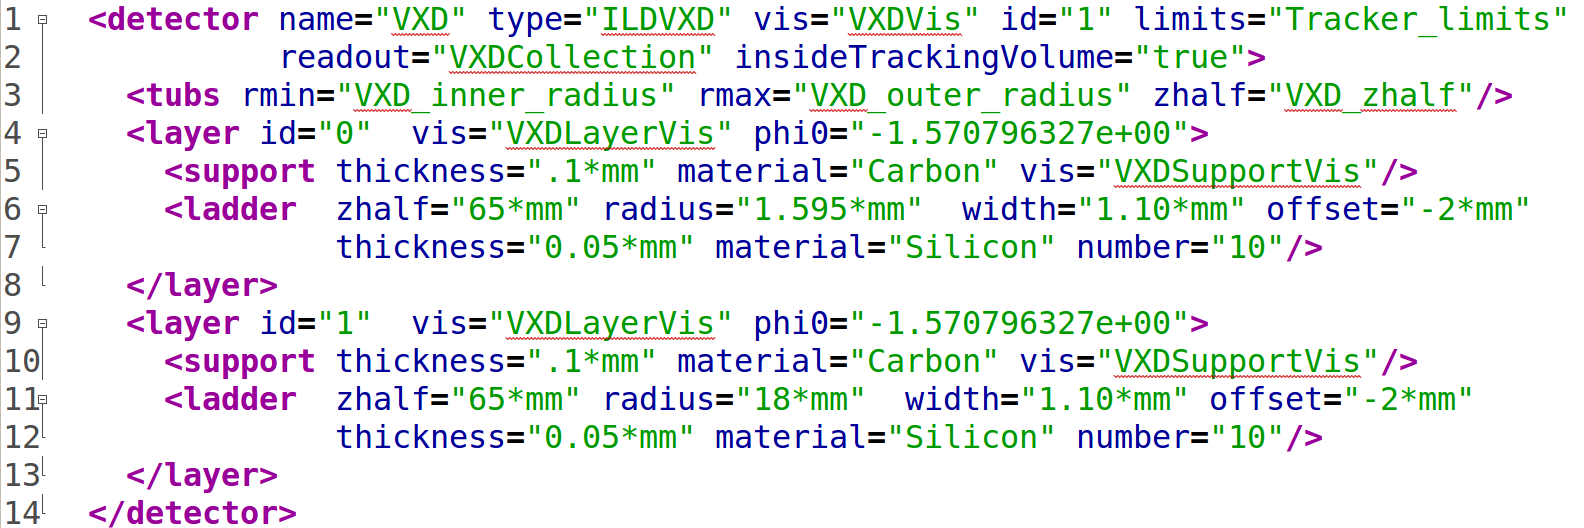
\includegraphics[width=16cm] {DD4hep_compact_xml.png}
%    \caption{An example sniplett of the compact detector description. The 
%             example shows the description of a 2 layered silicon vertex 
%             detector.}
%    \label{fig:fig-vxd-xml}
%  \end{center}
%  \vspace{-0.6cm}
%\end{figure}
%=============================================================================

%=============================================================================
\subsubsection{Detector Constructors}
\label{sec:detector-constructors}
%=============================================================================
\noindent
Detector Constructors are relatively small code fragments that get
as input an XML element from the compact description that represents 
a single detector instance. The code interprets the data and expands 
its geometry model in memory using the elements from the generic detector 
description model described in section~\ref{subsec:generic-model}.
The toolkit invokes these code fragments in a data driven way
using naming conventions during the initialization phase of the 
application. Users focus on one 
single detector type at the time, but the toolkit supports them to still
construct complex and large detector setups. 
Two implementations are currently supported: One is based on 
C++, which performs better and is able to detect errors at 
compiler time, but the code is slightly more technical.
The other is based on Python fragments, the code is more readable and
compact but errors are only detected at execution time.

\noindent
The compact description together with the detector constructors are sufficient
to build the detector model and to visualize it. If during the lifetime of the
experiment the detector model changes, the corresponding constructors will 
need to be adapted accordingly. 
DD4hep provides already a palette of basic pre-implemented geometrical detector 
concepts to design experiments. In view of usage of DD4hep as a detector 
description toolkit, this library may in the future also adopt
generic designs of detector components created by end users e.g. during the design 
phase of future experiments.
%=============================================================================
\begin{figure}[t]
  \begin{center}
    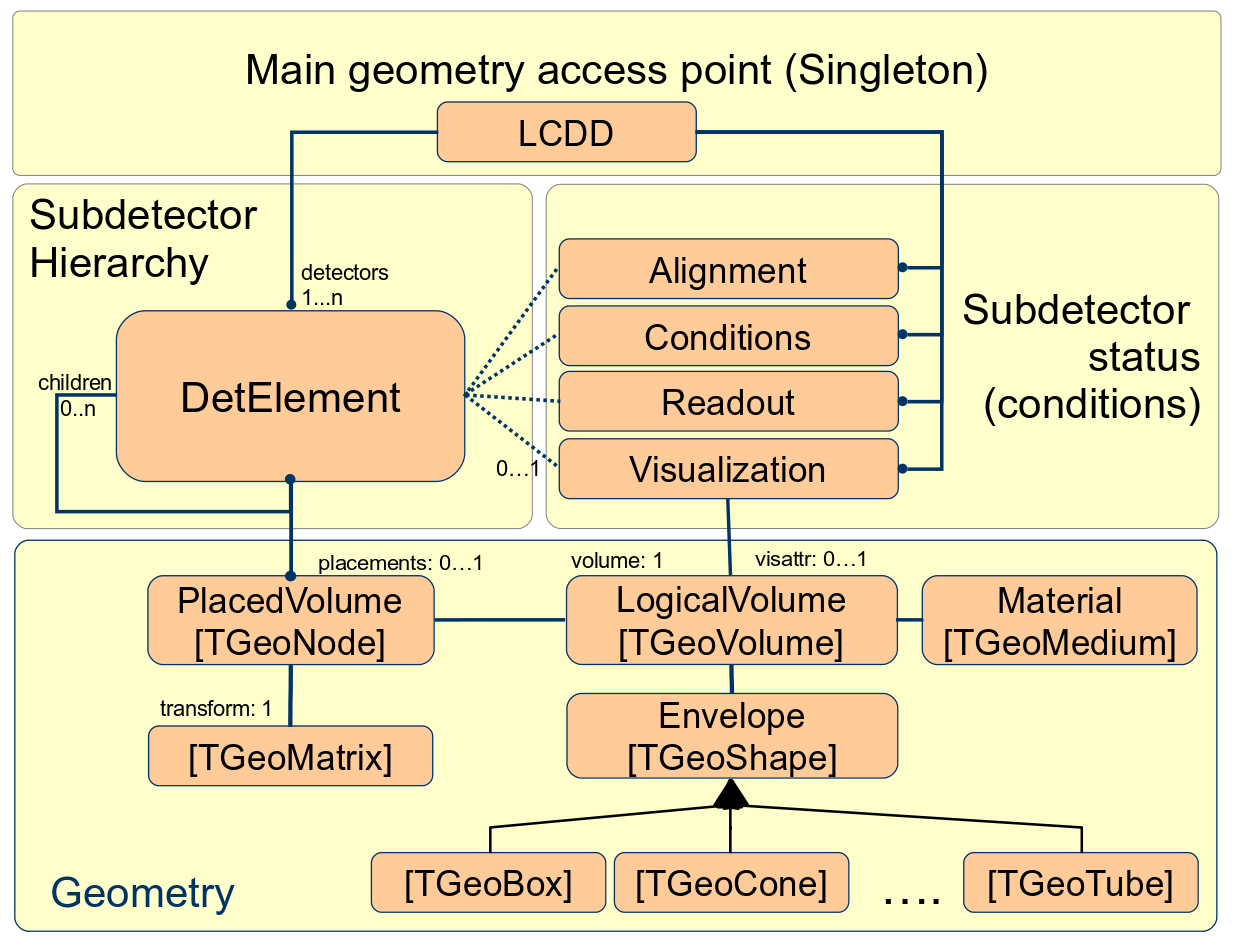
\includegraphics[height=110mm] {DD4hep_classes.png}
    \caption{Class diagram with the main classes and their relations 
             for the Generic Detector Description Model. The implementing
             ROOT classes are shown in brackets.}
    \label{fig:dd4hep-detector-model}
  \end{center}
\end{figure}
%=============================================================================
\subsection{Generic Detector Description Model}
\label{subsec:generic-model}
%=============================================================================

\noindent
This is the heart of the DD4hep detector description toolkit. Its purpose is 
to build in memory a model of the detector including its geometrical aspects
as well as structural and functional aspects. The design reuses the elements 
from the ROOT geometry package and extends them in case required functionality 
is not available. Figure~\ref{fig:dd4hep-detector-model} illustrates the main
players and their relationships.
Any detector is modeled as a tree of $Detector$ $Elements$, the entity 
central to this design, which is represented in the implementation by 
the $DetElement$ class~\cite{bib:LHCb-geometry}. It offers all
applications a natural entry point to any detector part of the experiment
and represents a complete sub-detector (e.g. TPC), a part of a 
sub-detector (e.g. TPC-Endcap), a detector module or any other convenient 
detector device. 
The main purpose is to give access to the data associated 
to the detector device. For example, if the user writes some TPC reconstruction 
code, accessing the TPC detector element from this code will provide access 
the all TPC geometrical dimensions, the alignment and calibration constants 
and other slow varying conditions such as the gas pressure, end-plate 
temperatures etc. The $Detector$ $Element$ acts as a data concentrator. 
Applications may access the full experiment geometry and all connected data
through a singleton object called $LCDD$, which provides 
management, bookkeeping and ownership to the model instances.

\noindent
The geometry is implemented using the ROOT geometry classes, which are used
directly without unnecessary interfaces to isolate the end-user from the 
actual ROOT based implementation. There is one exception: 
The constructors are wrapped to facilitate a very compact and readable 
notation to end-users building custom $Detector$ $Constructors$.

%=============================================================================
\subsubsection{Detector Element Tree versus the Geometry Hierarchy}
\label{subsect:detelement-hierarchy}
%=============================================================================
\noindent
The geometry part of the detector description is delegated to the ROOT classes.
$Logical$ $Volumes$ are the basic objects used in building the geometrical hierarchy. 
A $Logical$ $Volume$ is a shape with its dimensions and consist of a given material. 
They represent unpositioned objects which store all information about 
the placement of possibly embedded volumes. The same
volume can be replicated several times in the geometry. The $Logical$ $Volume$ also 
represents a system of reference with respect to its containing volumes.
The reuse of instances of $Logical$ $Volumes$ for different placements 
optimizes the memory consumption and detailed geometries for complex setups
consisting of millions of volumes may be realized with reasonable amount of memory.
The difficulty is to identify a given positioned volume 
in space and e.g. applying misalignment to one of these volumes. 
The relationship between the Detector Element and the placements
is not defined by a single reference to the placement, but the full path 
from the top of the detector geometry model to resolve existing
ambiguities due to the reuse of $Logical$ $Volumes$.
Hence, individual volumes must be identified by their full path from mother 
to daughter starting from the top-level volume. 

%=============================================================================
\begin{figure}[t]
  \begin{center}
    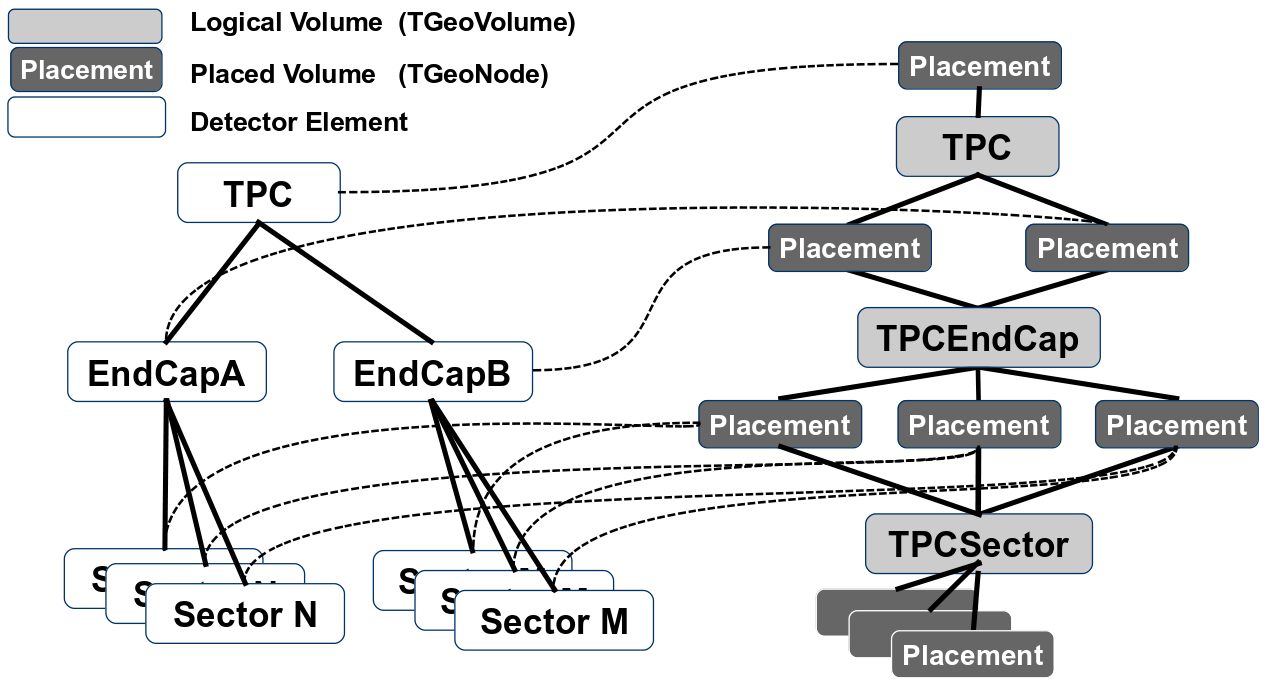
\includegraphics[height=85mm] {DD4hep_detelement_tree.png}
    \caption{The object diagram of a hypothetical TPC detector showing in
    parallel the $Detector$ $Element$ and the $Geometry$ hierarchy and the 
    relationships between the objects.}
    \label{fig:dd4hep-hierarchies}
  \end{center}
\end{figure}
%=============================================================================

\noindent
The tree structure of
Detector Elements is a parallel structure to the geometrical hierarchy.
This structure will probably not be as deep as the geometrical one since 
there would not need to associate detector information at very fine-grain 
level - it is unlikely that every little metallic screw
needs associated detector information such as alignment, conditions, etc.
Though this screw and many other replicas must be described in the geometry 
description since it may be important e.g. for its material contribution 
in the simulation application. Thus, the tree of Detector Elements is
fully degenerate and each detector element object will be placed only 
once in the detector element tree as illustrated for a hypothetical
TPC detector in Figure~\ref{fig:dd4hep-hierarchies}.

%=============================================================================
\subsubsection{Extensions and Views}
\label{subsect:extesions-and-views}
%=============================================================================

\noindent
As depicted in Figure~\ref{fig:dd4hep-big-picture} the reconstruction 
application will require special functionality extending the basics 
offered by the common detector element. This functionality may be
implemented by a set of specialized classes that will extend the 
detector element. These extensions will be in charge 
of providing specific answers to the questions formulated by the 
reconstruction algorithms such as pattern recognition, tracking, vertexing, 
particle identification, etc. One example could be to transform a calorimeter 
cell identifier into a 3D space position in the global coordinate system.
A generic detector description toolkit would be unable 
to answer this concrete question, however it provides a convenient 
environment for the developer to slot-in code fragments, which implement the
additional functionality using parameters stored
in the XML compact description.

\noindent
Depending on the functionality these specialized component must be able to
either store additional data, expose additional behavior or both. Additional 
behavior may easily be added overloading the $DetElement$ class using its 
internal data. The internal data is public and addressed by reference, hence
any number of views extending the $DetElement$ behavior may be constructed 
with very small overhead. Additional data may be added by any user at any time
to any instance of the $DetElement$ class using a simple aggregation 
mechanism shown in Figure~\ref{fig:dd4hep-extensions}. Data extensions must 
differ by their type. The freedom to attach virtually
any data item allows for optimized attachments depending on the 
application type, such as special attachments for reconstruction, 
simulation, tracking, etc.
%=============================================================================
\begin{figure}[t]
  \begin{center}
    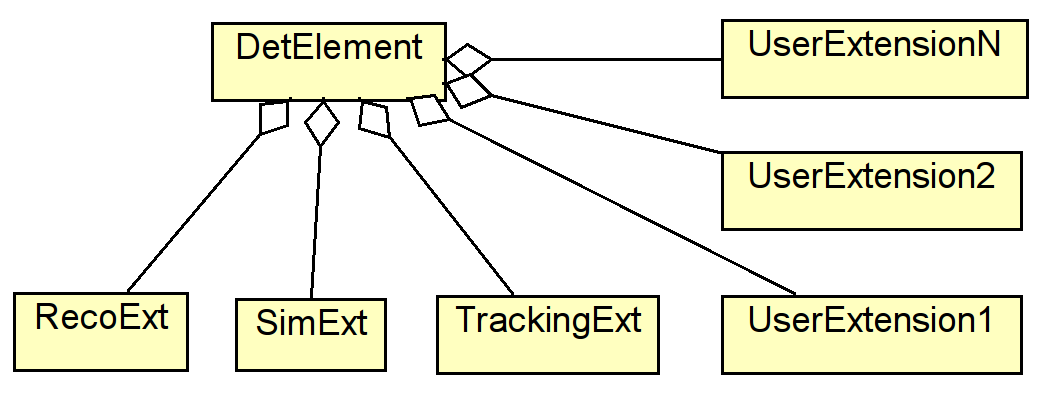
\includegraphics[width=115mm] {DD4hep-extensions.png}
    \caption{Extensions may be attached to common Detector Elements which 
             extend the functionality of the common DetElement 
             class and support e.g. caching of precomputed values.}
    \label{fig:dd4hep-extensions}
  \end{center}
\end{figure}
%=============================================================================
This design allows to build views addressing the following use-cases:
\begin{itemize}
\item{{\bf{Convenience Views}}} provide higher level abstractions
    and internally group complex calculations. Such views simplify 
    the life of the end-users.
\item{{\bf{Optimization Views}}} allows end-users extend the data of 
    the common detector detector element and store precomputed 
    results, which would be expensive to obtain repeatedly.
\item{{\bf{Compatibility Views}}} help to ensure smooth periods of 
    software redesign. During the life-time of the experiment
    often various software constructs are for functional reasons 
    re-designed and re-engineered.
    Compatibility Views either adapt new data designs to existing application 
    code or expose new behavior based on existing data.
\end{itemize}

%=============================================================================
\subsection{Simulation Support}
\label{subsect:simulation-support}
%=============================================================================
\noindent
Detector-simulation depends strongly on the use of an underlying simulation toolkit, 
the most prominent candidate nowadays being Geant4~\cite{bib:geant4}.
DD4hep supports simulation activities with Geant4 providing
an automatic translation mechanism between geometry representations.
The simulation response in the active elements of the detector
is not implemented by the toolkit, since it is strongly influenced by the technical 
choices and precise simulations depends on the very specific detection techniques.
In Geant4 this response is computed in software constructs called $Sensitive$ 
$Detectors$.

\noindent
Ideally DD4hep aims to provide a generic simulation application.
Similar to the palette of pre-implemented geometrical detector 
concepts to design experiments, it provides a palette of $Sensitive$
$Detectors$ to simulate the detector response in form of a component library.
Detector designers may base the simulation of a planned experiment 
on these predefined components for initial design and optimization 
studies.  In a similar way easy access
and configuration of other user actions of Geant4 is provided.

%=============================================================================
\subsection{Detector Alignment Support}
\label{subsect:alignment-support}
%=============================================================================
\noindent
The support for alignment operations is crucial to the usefulness of the
toolkit. In the linear collider community this support is basically missing 
in all the currently used geometry description systems.
The possibility to apply into the detector description alignment $deltas$ 
(differences with respect the ideal or measured position) and read them 
from an external source is mandatory to exploit the toolkit. A typical 
alignment application would consist of calculating a new set of $deltas$
from a given starting point, which could then be loaded and applied again 
in order to validate the alignment by recalculating some alignment residuals.
The ROOT geometry package supports to apply an [mis]-alignment to 
$touchable$ objects in the geometry. $Touchable$ objects are identified 
by the path of positioned volumes starting with the top node 
(e.g. path=$/TOP/A_1/B_4/C_3$). Contrary to ordinary multiple placements
of $Logical$ $Volumes$, $touchable$ objects are degenerate and only 
valid for one single volume~\cite{bib:ROOT-tgeo}. 
To simplify the usage for the end user,
the identification of a positioned volume will be connected
to the Detector Element, where only the relative path with respect 
to the Detector Element will have to be specified 
rather the full path from the top volume.
The $delta$-values will have to be read from various data sources.
The initial implementation will be based on simple XML files, later
a connection to other sources such as the detector conditions database
is envisaged.

